\documentclass[10pt,ignorenonframetext,]{beamer}
\setbeamertemplate{caption}[numbered]
\setbeamertemplate{caption label separator}{: }
\setbeamercolor{caption name}{fg=normal text.fg}
\beamertemplatenavigationsymbolsempty
\usepackage{lmodern}
\usepackage{amssymb,amsmath}
\usepackage{ifxetex,ifluatex}
\usepackage{fixltx2e} % provides \textsubscript
\ifnum 0\ifxetex 1\fi\ifluatex 1\fi=0 % if pdftex
  \usepackage[T1]{fontenc}
  \usepackage[utf8]{inputenc}
\else % if luatex or xelatex
  \ifxetex
    \usepackage{mathspec}
  \else
    \usepackage{fontspec}
  \fi
  \defaultfontfeatures{Ligatures=TeX,Scale=MatchLowercase}
\fi
\usetheme[]{Singapore}
\usefonttheme{serif}
% use upquote if available, for straight quotes in verbatim environments
\IfFileExists{upquote.sty}{\usepackage{upquote}}{}
% use microtype if available
\IfFileExists{microtype.sty}{%
\usepackage{microtype}
\UseMicrotypeSet[protrusion]{basicmath} % disable protrusion for tt fonts
}{}
\newif\ifbibliography
\hypersetup{
            pdftitle={Module 1: Introduction},
            pdfauthor={Stefanie Muff, Department of Mathematical Sciences, NTNU},
            colorlinks=true,
            linkcolor=Maroon,
            citecolor=Blue,
            urlcolor=blue,
            breaklinks=true}
\urlstyle{same}  % don't use monospace font for urls
\usepackage{color}
\usepackage{fancyvrb}
\newcommand{\VerbBar}{|}
\newcommand{\VERB}{\Verb[commandchars=\\\{\}]}
\DefineVerbatimEnvironment{Highlighting}{Verbatim}{commandchars=\\\{\}}
% Add ',fontsize=\small' for more characters per line
\usepackage{framed}
\definecolor{shadecolor}{RGB}{248,248,248}
\newenvironment{Shaded}{\begin{snugshade}}{\end{snugshade}}
\newcommand{\KeywordTok}[1]{\textcolor[rgb]{0.13,0.29,0.53}{\textbf{#1}}}
\newcommand{\DataTypeTok}[1]{\textcolor[rgb]{0.13,0.29,0.53}{#1}}
\newcommand{\DecValTok}[1]{\textcolor[rgb]{0.00,0.00,0.81}{#1}}
\newcommand{\BaseNTok}[1]{\textcolor[rgb]{0.00,0.00,0.81}{#1}}
\newcommand{\FloatTok}[1]{\textcolor[rgb]{0.00,0.00,0.81}{#1}}
\newcommand{\ConstantTok}[1]{\textcolor[rgb]{0.00,0.00,0.00}{#1}}
\newcommand{\CharTok}[1]{\textcolor[rgb]{0.31,0.60,0.02}{#1}}
\newcommand{\SpecialCharTok}[1]{\textcolor[rgb]{0.00,0.00,0.00}{#1}}
\newcommand{\StringTok}[1]{\textcolor[rgb]{0.31,0.60,0.02}{#1}}
\newcommand{\VerbatimStringTok}[1]{\textcolor[rgb]{0.31,0.60,0.02}{#1}}
\newcommand{\SpecialStringTok}[1]{\textcolor[rgb]{0.31,0.60,0.02}{#1}}
\newcommand{\ImportTok}[1]{#1}
\newcommand{\CommentTok}[1]{\textcolor[rgb]{0.56,0.35,0.01}{\textit{#1}}}
\newcommand{\DocumentationTok}[1]{\textcolor[rgb]{0.56,0.35,0.01}{\textbf{\textit{#1}}}}
\newcommand{\AnnotationTok}[1]{\textcolor[rgb]{0.56,0.35,0.01}{\textbf{\textit{#1}}}}
\newcommand{\CommentVarTok}[1]{\textcolor[rgb]{0.56,0.35,0.01}{\textbf{\textit{#1}}}}
\newcommand{\OtherTok}[1]{\textcolor[rgb]{0.56,0.35,0.01}{#1}}
\newcommand{\FunctionTok}[1]{\textcolor[rgb]{0.00,0.00,0.00}{#1}}
\newcommand{\VariableTok}[1]{\textcolor[rgb]{0.00,0.00,0.00}{#1}}
\newcommand{\ControlFlowTok}[1]{\textcolor[rgb]{0.13,0.29,0.53}{\textbf{#1}}}
\newcommand{\OperatorTok}[1]{\textcolor[rgb]{0.81,0.36,0.00}{\textbf{#1}}}
\newcommand{\BuiltInTok}[1]{#1}
\newcommand{\ExtensionTok}[1]{#1}
\newcommand{\PreprocessorTok}[1]{\textcolor[rgb]{0.56,0.35,0.01}{\textit{#1}}}
\newcommand{\AttributeTok}[1]{\textcolor[rgb]{0.77,0.63,0.00}{#1}}
\newcommand{\RegionMarkerTok}[1]{#1}
\newcommand{\InformationTok}[1]{\textcolor[rgb]{0.56,0.35,0.01}{\textbf{\textit{#1}}}}
\newcommand{\WarningTok}[1]{\textcolor[rgb]{0.56,0.35,0.01}{\textbf{\textit{#1}}}}
\newcommand{\AlertTok}[1]{\textcolor[rgb]{0.94,0.16,0.16}{#1}}
\newcommand{\ErrorTok}[1]{\textcolor[rgb]{0.64,0.00,0.00}{\textbf{#1}}}
\newcommand{\NormalTok}[1]{#1}
\usepackage{graphicx,grffile}
\makeatletter
\def\maxwidth{\ifdim\Gin@nat@width>\linewidth\linewidth\else\Gin@nat@width\fi}
\def\maxheight{\ifdim\Gin@nat@height>\textheight0.8\textheight\else\Gin@nat@height\fi}
\makeatother
% Scale images if necessary, so that they will not overflow the page
% margins by default, and it is still possible to overwrite the defaults
% using explicit options in \includegraphics[width, height, ...]{}
\setkeys{Gin}{width=\maxwidth,height=\maxheight,keepaspectratio}

% Prevent slide breaks in the middle of a paragraph:
\widowpenalties 1 10000
\raggedbottom

\AtBeginPart{
  \let\insertpartnumber\relax
  \let\partname\relax
  \frame{\partpage}
}
\AtBeginSection{
  \ifbibliography
  \else
    \let\insertsectionnumber\relax
    \let\sectionname\relax
    \frame{\sectionpage}
  \fi
}
\AtBeginSubsection{
  \let\insertsubsectionnumber\relax
  \let\subsectionname\relax
  \frame{\subsectionpage}
}

\setlength{\parindent}{0pt}
\setlength{\parskip}{6pt plus 2pt minus 1pt}
\setlength{\emergencystretch}{3em}  % prevent overfull lines
\providecommand{\tightlist}{%
  \setlength{\itemsep}{0pt}\setlength{\parskip}{0pt}}
\setcounter{secnumdepth}{0}
\usepackage{multirow}

\title{Module 1: Introduction}
\subtitle{TMA4268 Statistical Learning V2020}
\author{Stefanie Muff, Department of Mathematical Sciences, NTNU}
\date{6th January, 2020}

\begin{document}
\frame{\titlepage}

\begin{frame}

Last changes: 06.01.2020

\end{frame}

\begin{frame}{Acknowledgements}

This course had been built up by Mette Langaas at NTNU in 2018 and 2019.
I am using a lot of her material, and material from her TAs, throughout
the course.

\textbf{I would like to thank Mette for her great work and for the
permission to use her material!}

\end{frame}

\begin{frame}{Learning outcomes of TMA4268}

\begin{enumerate}
\def\labelenumi{\arabic{enumi}.}
\item
  \textbf{Knowledge.} The student has knowledge about the most popular
  statistical learning models and methods that are used for
  \emph{prediction} and \emph{inference} in science and technology.
  Emphasis is on regression- and classification-type statistical models.
\item
  \textbf{Skills.} The student can, based on an existing data set,
  choose a suitable statistical model, apply sound statistical methods,
  and perform the analyses using statistical software. The student can
  present, interpret and communicate the results from the statistical
  analyses, and knows which conclusions can be drawn from the analyses,
  and what are the caveats.
\end{enumerate}

\end{frame}

\begin{frame}{Learning material}

\begin{enumerate}
\def\labelenumi{\arabic{enumi})}
\item
  \textbf{The main learning source is the textbook by James, Witten, Hastie, Tibshirani (2013)}:
  ``An Introduction to Statistical Learning''. The textbook can be
  downloaded here: \url{https://www-bcf.usc.edu/~gareth/ISL/}

  \begin{itemize}
  \item
    The ebook an also be downloaded from Springer:
    \url{https://www.springer.com/gp/book/9781461471370} (NB, need to be
    on NTNU network or via vpn.)
  \item
    There are 15 hours of youtube videos by two of the authors of the
    book, Trevor Hastie an Rob Tibshirani -the inventors of statistical
    learning - all links
    \href{https://www.r-bloggers.com/in-depth-introduction-to-machine-learning-in-15-hours-of-expert-videos/}{here}
  \end{itemize}
\item
  All the lecture notes, \textbf{including any classnotes} made on the
  board (not necessarily available online).
\item
  \textbf{Additional reading material will be clearly indicated in the modules and on the course page.}
\end{enumerate}

\end{frame}

\begin{frame}{Course page}

All the relevant information for the course can be found here:

\url{https://wiki.math.ntnu.no/tma4268/2020v/start}

On each module page, all the relevant learning material and exercises
(incl. solutions) will be provided in due time.

\end{frame}

\begin{frame}{The Statistical Learning Team 2020}

\begin{block}{The TAs:}

\begin{itemize}
\tightlist
\item
  \href{https://www.ntnu.no/ansatte/martina.hall}{Martina Hall}; PhD
  student
\item
  \href{https://www.ntnu.no/ansatte/michail.spitieris}{Michail
  Spitieris}; PhD student
\end{itemize}

\end{block}

\begin{block}{The Lecturers}

\begin{itemize}
\tightlist
\item
  \href{https://www.ntnu.edu/employees/stefanie.muff}{Stefanie Muff};
  Associate Professor
\item
  \href{https://www.ntnu.no/ansatte/thiago.guerrera}{Thiago Guerrera
  Martins}; NTNU/AIAscience (Modules 6 \& 10)
\item
  \href{https://www.ntnu.no/ansatte/andreas.strand}{Andreas Strand}; PhD
  student (Module 7)
\end{itemize}

\end{block}

\end{frame}

\begin{frame}{Who is this course for?}

\begin{block}{Primary requirements}

\begin{itemize}
\item
  Bachelor level: 3rd year student from Science or Technology programs,
  and master/PhD level students with interest in performing statistical
  analyses.
\item
  Statistics background: TMA4240/45 Statistics, ST1101+ST1201
  (probability theory and statistical methods), or equivalent.
\item
  No background in statistical software needed: but we will use the R
  statistical software extensively in the course. Knowing python will
  make this easier for you!
\item
  Not a prerequisist but a good thing with knowledge of computing -
  preferably an introductory course in informatics, like TDT4105 or
  TDT4110.
\end{itemize}

\end{block}

\end{frame}

\begin{frame}

\begin{block}{Overlap}

\vspace{2mm}

\begin{itemize}
\item
  \href{https://www.ntnu.no/studier/emner/TDT4173\#tab=omEmnet}{TDT4173}
  Machine learning and case based reasoning: courses differ in
  philosophy (computer science vs.~statistics).
\item
  \href{https://www.ntnu.no/studier/emner/TMA4267\#tab=omEmnet}{TMA4267}
  Linear Statistical Models: useful to know about multivariate random
  vectors, covariance matrices and the multivariate normal distribution.
  Overlap only for Multiple linear regression (M3).
\end{itemize}

\end{block}

\end{frame}

\begin{frame}{About the course}

\begin{block}{Focus: Statistical theory \textbf{and} doing analyses}

\begin{itemize}
\item
  The course has focus on \textbf{statistical theory}, but we apply all
  models and theory using (mostly) available function in R and real data
  sets.
\item
  It is important that the student in the end of the course \textbf{can
  analyse all types of data} (covered in the course) - not just
  understand the theory.
\item
  And vice versa - the student must also \textbf{understand} the model,
  methods and algorithms used.
\end{itemize}

\end{block}

\end{frame}

\begin{frame}

\begin{block}{Teaching philosophy}

~

\begin{itemize}
\tightlist
\item
  Divide the topics of the course into modular units with specific
  focus.
\end{itemize}

~

\begin{itemize}
\tightlist
\item
  This (hopefully) facilitates learning?
\end{itemize}

~

\begin{itemize}
\tightlist
\item
  Two weeks without lectures (but supervision of exercises)
\end{itemize}

\end{block}

\end{frame}

\begin{frame}

\begin{block}{Course content: The 12 Modules}

\vspace{2mm}

\begin{itemize}
\tightlist
\item
  \textbf{Module 1}: Introduction (this module)
\item
  \textbf{Modules 2 - 11}:

  \begin{enumerate}
  \def\labelenumi{\arabic{enumi})}
  \setcounter{enumi}{1}
  \tightlist
  \item
    Statistical learning
  \item
    Multiple linear regression
  \item
    Classification
  \item
    Resampling methods
  \item
    Model selection/regularization
  \item
    Non-linearity
  \item
    Support vector machines
  \item
    Tree-based methods
  \item
    Unsupervised methods
  \item
    Neural nets
  \end{enumerate}
\item
  \textbf{Module 12}: Summing up
\end{itemize}

\end{block}

\end{frame}

\begin{frame}

\begin{block}{Learning methods, activities and grading}

\(~\)

\begin{itemize}
\tightlist
\item
  Lectures, exercises and works (projects).
\end{itemize}

~

\begin{itemize}
\tightlist
\item
  Portfolio assessment is the basis for the grade awarded in the course.
  This portfolio comprises

  \begin{itemize}
  \tightlist
  \item
    a written final examination (80\%).
  \item
    works (projects) (\(2\times 10\%=20\%\)).
  \end{itemize}
\end{itemize}

~

\begin{itemize}
\tightlist
\item
  The results for the constituent parts are to be given in \%-points,
  while the grade for the whole portfolio (course grade) is given by the
  letter grading system. Retake of examination may be given as an oral
  examination. The lectures are given in English.
\end{itemize}

\end{block}

\end{frame}

\begin{frame}

\begin{block}{The lectures}

\vspace{2mm}

\textbf{Mondays at 10.15-12.00 in S1 and Fridays at 14.15-16.00 in S4}

\begin{itemize}
\item
  We have \(2\cdot 2\) hours of lectures every week (except when working
  with the compulsory exercises).
\item
  \textbf{Note}: The \textbf{first lecture of each module will be on
  Fridays}, the second lecture on \textbf{Mondays}, and the exercise
  that corresponds to this module on Thursdays. See
  \href{https://github.com/stefaniemuff/statlearning/blob/master/TMA4268_schedule2020.pdf}{here}
  for a tentative schedule.
\item
  Some weeks the Monday lecture will be \emph{interactive} or with some
  self-study / exercise component, where
  \emph{\textcolor{red}{active learning}} is in focus.
\item
  The other weeks (modules 3, 4, 6, 8, 10 and 11) the Monday lecture is
  a plenary lecture in S1.
\item
  \textbf{I suggest that you always bring your laptop to the Monday
  lecture.}
\item
  In the \textbf{first week of the course} we need time for an R
  workshop!
\end{itemize}

\end{block}

\end{frame}

\begin{frame}

\begin{block}{The weekly supervision sessions}

~

\textbf{Thursdays 08.15-10:00 in Smia} ~\\
\hspace*{0.333em}

\begin{itemize}
\item
  For each module \emph{recommended exercises} are uploaded. These are
  partly

  \begin{itemize}
  \tightlist
  \item
    theoretical exercises (from book or not)
  \item
    computational tasks
  \item
    data analysis
  \end{itemize}
\item
  These are supervised in the weekly exercise slots.
\item
  Solutions will be provided to check yourself (no grading).
\end{itemize}

\end{block}

\end{frame}

\begin{frame}

\begin{block}{The compulsory exercises}

\begin{itemize}
\item
  We will have \textbf{two compulsory exercises}, each with a maximal
  score of 50 points.
\item
  These are supervised in the weekly exercise slots and there will be
  one week without lectures (only with supervision) for each compulsory
  exercise.
\item
  Focus: theory, analysis in R, and interpretation.
\item
  Work in \textbf{groups of maximum 3}; handed in on Blackboard and be
  written in R Markdown (both .Rmd and .pdf handed in).
\item
  The TAs grade the exercises.
\item
  This gives 20\% of the final evaluation in the course, the written
  exam the remaining 80\%.
\end{itemize}

\end{block}

\end{frame}

\begin{frame}

\begin{itemize}
\tightlist
\item
  The \textbf{first compulsory exercises} will be held after Modules
  1-5.
\end{itemize}

\hspace{8mm} Suggested submission deadline:

\hspace{8mm} \textbf{Thursday, 20. Februar 2020, 12:00h}.

\vspace{8mm}

\begin{itemize}
\tightlist
\item
  The \textbf{second compulsory exercise} will be held after Modules
  6-11.
\end{itemize}

\hspace{8mm}Suggested submission deadline:

\hspace{8mm}\textbf{Monday, 13. April 2020, 12:00h}.

\end{frame}

\begin{frame}

\begin{block}{Tentative schedule}

\vspace{2mm}

A tentative schedule (i.e., with continous updates) can be found under
the following link (als available from our course page):

\vspace{2mm}

\url{https://github.com/stefaniemuff/statlearning/blob/master/TMA4268_schedule2020.pdf}

\end{block}

\end{frame}

\begin{frame}

\begin{block}{The lecture material}

\vspace{2mm}

\begin{itemize}
\item
  All the material presented in class will be available on our course
  webpage (\url{https://wiki.math.ntnu.no/tma4268/2020v/start}).
\item
  There will be both a .pdf and an .Rmd version of the lecture notes.
  This will allow you to check and use the code that I use to generate
  the slides.
\item
  For exercises, we provide a .pdf, .Rmd and an .html version.
\end{itemize}

\end{block}

\end{frame}

\begin{frame}{Student active learning}

Student's learning styles are different! Felder and Silverman (1988)
suggested the following learning style axes:

\begin{enumerate}
\def\labelenumi{\arabic{enumi})}
\item
  \textbf{active - reflective}: How do you process information: actively
  (through physical activities and discussions), or reflexively (through
  introspection)?
\item
  \textbf{sensing-intuitive}: What kind of information do you tend to
  receive: sensitive (external agents like places, sounds, physical
  sensation) or intuitive (internal agents like possibilities, ideas,
  through hunches)?
\item
  \textbf{visual-verbal:} Through which sensorial channels do you tend
  to receive information more effectively: visual (images, diagrams,
  graphics), or verbal (spoken words, sound)? Many students have a
  visual learning style!
\item
  \textbf{sequential - global}: How do you make progress: sequentially
  (with continuous steps), or globally (through leaps and an integral
  approach)?
\end{enumerate}

\end{frame}

\begin{frame}

\begin{block}{We try!}

\vspace{2mm}

\begin{itemize}
\item
  \(\ldots\) to acknowledging these different learning style axes.
\item
  \(\ldots\) to choose teaching styles that match the learning styles of
  as many students as possible.
\end{itemize}

\vspace{-3mm}

\begin{itemize}
\item
  \(\ldots\) to provide learning environments, opportunities,
  interactions, and tasks that help to learn deeper.
\item
  \(\ldots\) to provide guidance and support that challenges students
  based on their current ability.
\end{itemize}

We will now focus on \emph{active} and \emph{reflective} learning styles
and learning methods.

\end{block}

\end{frame}

\begin{frame}

\begin{block}{Active vs.~reflective learning styles}

\vspace{2mm}

\textbf{Reflective learning methods}

\begin{itemize}
\tightlist
\item
  Plenary lectures
\item
  Reading textbook
\item
  Self study
\end{itemize}

\vspace{4mm}

\textbf{Active learing methods}

\begin{itemize}
\tightlist
\item
  Pause in plenary lecture to ask questions and let students think
  and/or discuss.
\item
  In-class quizzes 
\item
  Projects - individual or in groups
\item
  Group discussion
\item
  Interactive lectures
\end{itemize}

\end{block}

\end{frame}

\begin{frame}{Test your learning style}

\vspace{2mm}

If you are interested in your learning style, we are very grateful if
you can fill out this questionnaire:

\url{https://innsida.ntnu.no/forms/view.php?id=221738}

\begin{itemize}
\tightlist
\item
  The intro is in Norwegian.
\item
  The questionnaire is in English.
\item
  If you have questions, contact Mettee Langaas
  (\href{mailto:mette.langaas@ntnu.no}{\nolinkurl{mette.langaas@ntnu.no}}).
\item
  You will get an email with your results.
\item
  We have been given permission to collect these data for research.
\end{itemize}

\end{frame}

\begin{frame}{Who are you - and what are your expectations?}

~

In class - go to \url{https://app.klicker.uzh.ch/join/bkx} to answer
these questions.

\end{frame}

\begin{frame}{Reference group}

\textbf{At least 3 members, ideally one from different programmes}

\begin{itemize}
\tightlist
\item
  At least one from IndMat, year 3
\item
  Any programme, year 4
\item
  Not IndMat
\end{itemize}

Volunteers?

\begin{itemize}
\tightlist
\item
  Andreas Matre,
  \href{mailto:andrmatr@stud.ntnu.no}{\nolinkurl{andrmatr@stud.ntnu.no}}
  (3 year Bachelor)
\item
  Sara Elise Wøllo,
  \href{mailto:saraew@stud.ntnu.no}{\nolinkurl{saraew@stud.ntnu.no}}
  (Industrial Mathematics)
\item
  John Lau,
  \href{mailto:johnlau@stud.ntnu.no}{\nolinkurl{johnlau@stud.ntnu.no}}
  (Other)
\end{itemize}

Thanks to the three people that volunteered.

\end{frame}

\begin{frame}{Module 1}

\begin{block}{Aims of the first module}

\begin{itemize}
\item
  An introduction to statistical learning. What is it?
\item
  Types of problems we will look at
\item
  \textbf{Introduction to R and RStudio } 
\end{itemize}

\end{block}

\end{frame}

\begin{frame}

\begin{block}{Learning material for this module}

\begin{itemize}
\item
  Our textbook James et al (2013): An Introduction to Statistical
  Learning - with Applications in R (ISL). Chapter 1 (Introduction) and
  2.3 (Lab: Introduction to R).
\item
  \href{https://htmlpreview.github.io/?https://github.com/stefaniemuff/statlearning/blob/master/Exercise1/Rbeginner.html}{\texttt{Rbeginner}},
  \href{https://htmlpreview.github.io/?https://github.com/stefaniemuff/statlearning/blob/master/Exercise1/Rintermediate.html}{\texttt{Rintermediate}},
  and
  \href{https://htmlpreview.github.io/?https://github.com/stefaniemuff/statlearning/blob/master/Exercise1/Rplots.html}{\texttt{Rplots}}
\end{itemize}

\vspace{3mm}

\emph{Recommended}:

\begin{itemize}
\item
  Watch the video lecture for Chapter 1 by Hastie and Tibshirani
  \href{https://www.r-bloggers.com/in-depth-introduction-to-machine-learning-in-15-hours-of-expert-videos/}{here}.
\item
  Background on Matrix Algebra:
  \href{https://link.springer.com/chapter/10.1007/978-3-662-45171-7_2}{Härdle
  and Simes (2015) - Chapter 2: A short excursion into Matrix Algebra}
  (on the reading list for TMA4267 Linear statistical models).
\end{itemize}

\end{block}

\end{frame}

\begin{frame}{What is statistical learning?}

\begin{itemize}
\tightlist
\item
  Refers to \emph{a vast set of tools to understanding data} (text book,
  p.~1).
\end{itemize}

\vspace{1mm}

\begin{itemize}
\tightlist
\item
  Main distinction: \emph{\textcolor{red}{Supervised}} versus
  \emph{\textcolor{red}{unsupervised learning}}.
\end{itemize}

\vspace{1mm}

\begin{itemize}
\tightlist
\item
  Both \textbf{prediction} and \textbf{understanding} (inference
  \(\rightarrow\) drawing conclusions).
\end{itemize}

\vspace{1mm}

\begin{itemize}
\tightlist
\item
  Statistical learning is \textbf{a statistical discipline}, but the
  boarders are becoming more blurred.
\end{itemize}

\end{frame}

\begin{frame}{Statistical Learning vs. ``Machine Learning''}

\vspace{2mm}

\begin{itemize}
\tightlist
\item
  Machine learning is more focused on the algorithmic part of learning,
  and is a \emph{discipline in computer science}.
\end{itemize}

\vspace{2mm}

\begin{itemize}
\tightlist
\item
  But many methods/algorithms are common to both fields.
\end{itemize}

\end{frame}

\begin{frame}{Statistical Learning vs. ``Data Science''}

Data science

\begin{itemize}
\item
  The aim is to extract knowledge and understanding from data.
  \vspace{2mm}
\item
  Requires a combination of statistics, mathematics, numerics, computer
  science and informatics.
\end{itemize}

This encompasses the whole process of data acquisition/scraping, going
from unstructured to structured data, setting up a data model,
performing data analysis, implementing tools and interpreting results.

In statistical learning we will not work on the two first above
(acquisition and unstructured to structured).

\href{http://r4ds.had.co.nz/}{R for Data Science} is an excellent read
and relevant for this course!

\end{frame}

\begin{frame}{Problems you will learn to solve}

There are \textbf{three main types of problems} discussed in this
course:

\begin{itemize}
\item
  Regression (supervised)
\item
  Classification (supervised)
\item
  Unsupervised methods
\end{itemize}

using data from science, technology, industry, economy/finance, \ldots{}

\end{frame}

\begin{frame}[fragile]{Example 1: Regression (Etiology of CVD)}

\begin{itemize}
\item
  The Framingham Heart Study investigates the underlying causes of
  cardiovascular disease (CVD) (see
  \url{https://www.framinghamheartstudy.org/}). 
\item
  Aim: modelling systolic blood pressure (\texttt{SYSBP}) using data
  from \(n=2600\) persons.
\item
  For each person in the data set we have measurements of the following
  seven variables.
\end{itemize}

\scriptsize

\begin{itemize}
\tightlist
\item
  \texttt{SYSBP} systolic blood pressure (mmHg),
\item
  \texttt{SEX} 1=male, 2=female,
\item
  \texttt{AGE} age (years),
\item
  \texttt{CURSMOKE} current cigarette smoking at examination: 0=not
  current smoker, 1= current smoker,
\item
  \texttt{BMI} body mass index,
\item
  \texttt{TOTCHOL} serum total cholesterol (mg/dl),
\item
  \texttt{BPMEDS} use of anti-hypertensive medication at examination:
  0=not currently using, 1=currently using. \normalsize
\end{itemize}

\end{frame}

\begin{frame}

\begin{center}\includegraphics[width=1\linewidth]{1Intro_files/figure-beamer/CVDread-1} \end{center}

What does this plot show?

Red: male; turquoise: female

\end{frame}

\begin{frame}

\begin{itemize}
\tightlist
\item
  Diagonal: density plot (generalization of histogram), or barplot.
\item
  Lower diagonals: scatterplot, histograms
\item
  Upper diagonals: correlations values, boxplots, barplots
\end{itemize}

\end{frame}

\begin{frame}

\begin{block}{Etiology of CVD}

\vspace{2mm}

The question: \textbf{What are the factors that cause high SBP?}

\vspace{2mm}

So we are interested in \emph{inference} (explanation) and not
predction!

\vspace{4mm}

\begin{itemize}
\item
  A \emph{multiple normal linear regression model} was fit to the data
  set with \[-\frac{1}{\sqrt{\texttt{SYSBP}}}\] as response (output) and
  all the other variables as covariates (inputs).
\item
  The results are used to formulate hypotheses about the etiology of CVD
  - to be studied in new trials.
\end{itemize}

\end{block}

\end{frame}

\begin{frame}[fragile]

\scriptsize

\begin{Shaded}
\begin{Highlighting}[]
\NormalTok{modelB =}\StringTok{ }\KeywordTok{lm}\NormalTok{(}\OperatorTok{-}\DecValTok{1}\OperatorTok{/}\KeywordTok{sqrt}\NormalTok{(SYSBP) }\OperatorTok{~}\StringTok{ }\NormalTok{SEX }\OperatorTok{+}\StringTok{ }\NormalTok{AGE }\OperatorTok{+}\StringTok{ }\NormalTok{CURSMOKE }\OperatorTok{+}\StringTok{ }\NormalTok{BMI }\OperatorTok{+}\StringTok{ }\NormalTok{TOTCHOL }\OperatorTok{+}\StringTok{ }\NormalTok{BPMEDS, }
    \DataTypeTok{data =}\NormalTok{ thisds)}

\KeywordTok{summary}\NormalTok{(modelB)}
\end{Highlighting}
\end{Shaded}

\begin{verbatim}
## 
## Call:
## lm(formula = -1/sqrt(SYSBP) ~ SEX + AGE + CURSMOKE + BMI + TOTCHOL + 
##     BPMEDS, data = thisds)
## 
## Residuals:
##        Min         1Q     Median         3Q        Max 
## -0.0207366 -0.0039157 -0.0000304  0.0038293  0.0189747 
## 
## Coefficients:
##               Estimate Std. Error t value Pr(>|t|)    
## (Intercept) -1.106e-01  1.342e-03 -82.413  < 2e-16 ***
## SEX2        -2.989e-04  2.390e-04  -1.251 0.211176    
## AGE          2.378e-04  1.434e-05  16.586  < 2e-16 ***
## CURSMOKE1   -2.504e-04  2.527e-04  -0.991 0.321723    
## BMI          3.087e-04  2.955e-05  10.447  < 2e-16 ***
## TOTCHOL      9.288e-06  2.602e-06   3.569 0.000365 ***
## BPMEDS1      5.469e-03  3.265e-04  16.748  < 2e-16 ***
## ---
## Signif. codes:  0 '***' 0.001 '**' 0.01 '*' 0.05 '.' 0.1 ' ' 1
## 
## Residual standard error: 0.005819 on 2593 degrees of freedom
## Multiple R-squared:  0.2494, Adjusted R-squared:  0.2476 
## F-statistic: 143.6 on 6 and 2593 DF,  p-value: < 2.2e-16
\end{verbatim}

\normalsize

\end{frame}

\begin{frame}[fragile]{Example 2: Classification (iris plants)}

The \texttt{iris} flower data set is a very famous multivariate data set
introduced by the British statistician and biologist Ronald Fisher in
1936.

\(~\)

The data set contains

\begin{itemize}
\tightlist
\item
  \textbf{three plant species} \{setosa, virginica, versicolor\}
\item
  \textbf{four features measured} for each corresponding sample:

  \begin{itemize}
  \tightlist
  \item
    \texttt{Sepal.Length}
  \item
    \texttt{Sepal.Width}
  \item
    \texttt{Petal.Length}
  \item
    \texttt{Petal.Width}.
  \end{itemize}
\end{itemize}

\end{frame}

\begin{frame}

\begin{figure}
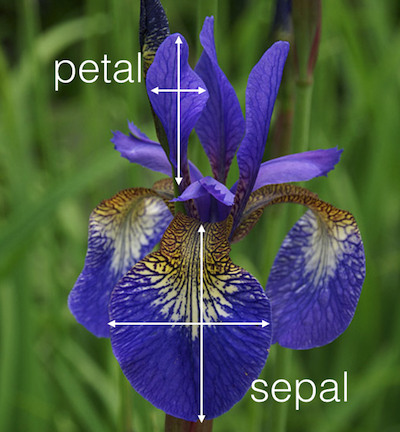
\includegraphics[width=150pt]{iris} \caption{Iris plant with sepal and petal leaves}\label{fig:iris_pic}
\end{figure}

\tiny
<http://blog.kaggle.com/2015/04/22/scikit-learn-video-3-machine-learning-first-steps-with-the-iris-dataset/>

\end{frame}

\begin{frame}[fragile]

\scriptsize

\begin{Shaded}
\begin{Highlighting}[]
\KeywordTok{head}\NormalTok{(iris)}
\end{Highlighting}
\end{Shaded}

\begin{verbatim}
##   Sepal.Length Sepal.Width Petal.Length Petal.Width Species
## 1          5.1         3.5          1.4         0.2  setosa
## 2          4.9         3.0          1.4         0.2  setosa
## 3          4.7         3.2          1.3         0.2  setosa
## 4          4.6         3.1          1.5         0.2  setosa
## 5          5.0         3.6          1.4         0.2  setosa
## 6          5.4         3.9          1.7         0.4  setosa
\end{verbatim}

\normalsize

\end{frame}

\begin{frame}

Aim: correctly classify the species of an iris plant from sepal length
and sepal width.

\includegraphics{1Intro_files/figure-beamer/iriscont-1.pdf}

\end{frame}

\begin{frame}

\begin{block}{Linear boundaries}

\vspace{1mm}

In this plot the small black dots represent correctly classified iris
plants, while the red dots represent misclassifications. The big black
dots represent the class means.

~

\includegraphics[width=10cm]{1Intro_files/figure-beamer/irislda-1}

\end{block}

\end{frame}

\begin{frame}

\begin{block}{Non-linear boundaries}

\vspace{1mm}

Sometimes a more suitable boundary is not linear.\\
\hspace*{0.333em}

\includegraphics[width=10cm]{1Intro_files/figure-beamer/irisqda-1}

\end{block}

\end{frame}

\begin{frame}{Example 3: Unsupervised methods (Gene expression)}

\begin{itemize}
\tightlist
\item
  In a collaboration with researchers the Faculty of Medicine and Health
  the relationship between inborn maximal oxygen uptake and skeletal
  muscle gene expression was studied.
\item
  Rats were artificially selected for high- and low running capacity
  (HCR and LCR, respectively),
\item
  Rats were either kept seditary or trained.
\item
  Transcripts significantly related to running capacity and training
  were identified. 
\item
  To further present the findings heat map of the most significant
  transcripts were presented (high expression are shown in red and
  transcripts with a low expression are shown in yellow).
\item
  This is hierarchical cluster analysis with pearson correlation
  distance measure.
\end{itemize}

\end{frame}

\begin{frame}

\begin{figure}
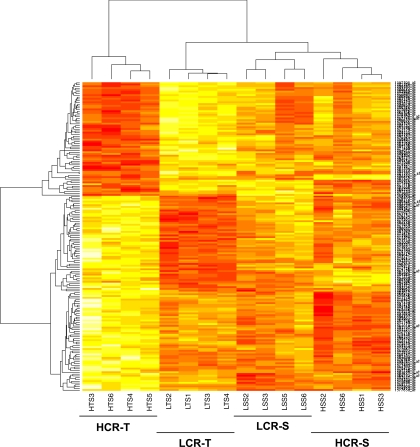
\includegraphics[width=150pt]{heatmap} \caption{Heat map of the most significant transcripts. Transcripts with a high expression are shown in red and transcripts with a low expression are shown in yellow.}\label{fig:heatmap_pic}
\end{figure}

\tiny
More: \url{https://www.ncbi.nlm.nih.gov/pmc/articles/PMC2585023/}

\end{frame}

\begin{frame}{Example 4: Unsupervised methods (Network clustering)}

\vspace{2mm}

Finding clusters in protein-protein-interaction networks. \vspace{2mm}

\includegraphics{muff_etal.png}

\end{frame}

\begin{frame}{Plan for this week}

\begin{block}{Thursday January 9, 8.15-10.00 in Smia}

\begin{itemize}
\item
  Workshop for R and RStudio
\item
  Stefanie, Martina and Michail present
\end{itemize}

\vspace{4mm}

\end{block}

\begin{block}{Friday January 10, 14.15-16.00 in S4}

\begin{itemize}
\tightlist
\item
  Lecture 1 of Module 2
\end{itemize}

\end{block}

\end{frame}

\begin{frame}{Getting started with R}

\vspace{2mm}

\begin{itemize}
\tightlist
\item
  Install R (use the Norwegian CRAN mirror):
  \url{https://www.r-project.org}
\end{itemize}

\vspace{2mm}

\begin{itemize}
\tightlist
\item
  Install Rstudio \url{https://www.rstudio.com/products/rstudio/}
\end{itemize}

\vspace{4mm}

If you need help on installing R and RStudio on you laptop computer,
contact \href{mailto:orakel@ntnu.no}{\nolinkurl{orakel@ntnu.no}}.

\end{frame}

\begin{frame}

\begin{block}{R, Rstudio, CRAN and GitHub}

\vspace{2mm}

\begin{enumerate}
\def\labelenumi{\arabic{enumi})}
\item
  What is R? \url{https://www.r-project.org/about.html} \vspace{2mm}
\item
  What is RStudio? \url{https://www.rstudio.com/products/rstudio/}
  \vspace{2mm}
\item
  What is CRAN? \url{https://cran.uib.no/} \vspace{2mm}
\item
  What is GitHub and Bitbucket? Do we need GitHub or Bitbucket in our
  course? \url{https://www.youtube.com/watch?v=w3jLJU7DT5E} and
  \url{https://techcrunch.com/2012/07/14/what-exactly-is-github-anyway/}
\end{enumerate}

\end{block}

\end{frame}

\begin{frame}

\begin{block}{Getting to work with RStudio}

\vspace{6mm}

\(\rightarrow\) Short demo in class.

\end{block}

\end{frame}

\begin{frame}

\begin{block}{A first look at R and RStudio}

\vspace{6mm}

\begin{itemize}
\tightlist
\item
  \href{https://github.com/stefaniemuff/statlearning/blob/master/1Intro/Rbeginner.pdf}{Rbeginner.pdf}
\item
  \href{https://github.com/stefaniemuff/statlearning/blob/master/1Intro/Rbeginner.Rmd}{Rbeginner.Rmd}
\end{itemize}

\end{block}

\end{frame}

\begin{frame}

\begin{block}{A second look at R and probability distributions}

\vspace{6mm}

\begin{itemize}
\tightlist
\item
  \href{https://github.com/stefaniemuff/statlearning/blob/master/1Intro/Rintermediate.pdf}{Rintermediate.pdf}
\item
  \href{https://github.com/stefaniemuff/statlearning/blob/master/1Intro/Rintermediate.Rmd}{Rintermediate.Rmd}
\end{itemize}

To see solutions added to the files, add -sol to filename to get

\begin{itemize}
\tightlist
\item
  \href{https://github.com/stefaniemuff/statlearning/blob/master/1Intro/Rintermediate-sol.html}{Rintermediate-sol.html}
\end{itemize}

\end{block}

\end{frame}

\begin{frame}

\begin{block}{And resources about plots}

\vspace{6mm}

\begin{itemize}
\tightlist
\item
  \href{https://github.com/stefaniemuff/statlearning/blob/master/1Intro/Rplots.pdf}{Rplots.pdf}
\item
  \href{https://github.com/stefaniemuff/statlearning/blob/master/1Intro/Rplots.Rmd}{Rplots.Rmd}
\end{itemize}

To see solutions added to the files, add -sol to filename to get

\begin{itemize}
\tightlist
\item
  \href{https://github.com/stefaniemuff/statlearning/blob/master/1Intro/Rplots-sol.html}{Rplots-sol.html}
\end{itemize}

\end{block}

\end{frame}

\begin{frame}

\begin{block}{Additional nice R resources}

\vspace{2mm}

\begin{itemize}
\tightlist
\item
  P. Dalgaard: Introductory statistics with R, 2nd edition, Springer,
  which is also available freely to NTNU students as an ebook:
  \href{https://link.springer.com/book/10.1007/978-0-387-79054-1}{Introductory
  Statistics with R}.
\end{itemize}

\vspace{1mm}

\begin{itemize}
\tightlist
\item
  Grolemund and Hadwick (2017): ``R for Data Science'',
  \url{http://r4ds.had.co.nz}
\end{itemize}

\vspace{1mm}

\begin{itemize}
\tightlist
\item
  Hadwick (2009): ``ggplot2: Elegant graphics for data analysis''
  textbook: \url{https://ggplot2-book.org/}
\end{itemize}

\vspace{1mm}

\begin{itemize}
\tightlist
\item
  \href{https://www.rstudio.com/resources/cheatsheets/}{Overview of
  cheat sheets from RStudio}
\end{itemize}

\begin{itemize}
\tightlist
\item
  Questions on R: ask the course staff, colleagues, and
  \href{https://stackoverflow.com/}{stackoverflow}.
\end{itemize}

\end{block}

\end{frame}

\begin{frame}{Acknowledgements}

Thanks to Julia Debik for contributing to this module page.

\end{frame}

\begin{frame}{Supplement: Exam from 2019}

This is the digital exam held in Inspera.

\begin{itemize}
\tightlist
\item
  \href{https://www.math.ntnu.no/emner/TMA4268/Exam/V2019e.pdf}{Problem
  set}
\item
  \href{https://www.math.ntnu.no/emner/TMA4268/Exam/e2019sol.html}{Tentative
  solutions}
\item
  \href{https://www.math.ntnu.no/emner/TMA4268/Exam/gradingdocumentV2019.pdf}{Grading
  document}
\end{itemize}

However, please note that this was the exam created by Mette Langaas and
her team, and not by us. The recommended and compulsory exercises will
give you hints abou the exam, so we highly recommend you will work on
them.

\end{frame}

\end{document}
